\documentclass[aspectratio=169]{beamer}
\usepackage{beamerthemesplit}
\usepackage{multirow}
\usepackage{array}
\usepackage{hyperref}
\usepackage[T1]{fontenc}
\usepackage{inconsolata}
\usepackage{xcolor,colortbl}
\usepackage{natbib}
\usepackage{listings}
%%\newcommand{\newblock}{}
\DeclareGraphicsExtensions{.pdf,.png,.jpg}
\usetheme[pageofpages=of,% String used between the current page and the
                         % total page count.
          bullet=circle,% Use circles instead of squares for bullets.
          titleline=true,% Show a line below the frame title.
          alternativetitlepage=true,% Use the fancy title page.
          ]{Torino}
\definecolor{light-green}{RGB}{144,238,144}
\makeatletter
\setbeamertemplate{footline}
{
  \leavevmode%
  \hbox{%
  \begin{beamercolorbox}[wd=.333333\paperwidth,ht=2.25ex,dp=1ex,center]{author in head/foot}%
    \usebeamerfont{author in head/foot}\insertshortauthor~~\beamer@ifempty{\insertshortinstitute}{}{(\insertshortinstitute)}
  \end{beamercolorbox}%
  \begin{beamercolorbox}[wd=.333333\paperwidth,ht=2.25ex,dp=1ex,center]{title in head/foot}%
    \usebeamerfont{title in head/foot}\insertshorttitle
  \end{beamercolorbox}%
  \begin{beamercolorbox}[wd=.333333\paperwidth,ht=2.25ex,dp=1ex,right]{date in head/foot}%
    \usebeamerfont{date in head/foot}\insertshortdate{}\hspace*{2em}
%    \insertframenumber{} / \inserttotalframenumber\hspace*{2ex} % DELETED
  \end{beamercolorbox}}%
  \vskip0pt%
}
\makeatother
\begin{document}
\author{{\bf Casey Stella}\\@casey\_stella}
\institute[Hortonworks]{
\includegraphics[width=40px,height=17px]{logo}}
\title{{\bf Apache Metron }}
\subtitle{{\bf Lessons Learned}}
\date{2018} 

\frame{\titlepage} 

\begingroup
\Huge
\begin{frame}
\frametitle{Introduction}
\begin{center}
Hi, I'm Casey Stella!
\end{center}
\end{frame}
\endgroup

\section{Apache Metron}

\frame{\frametitle{Apache Metron: A Cybersecurity Analytics Platform}
\begin{itemize}
\item Metron provides a scalable, advanced security analytics framework to offer a centralized tool for security monitoring and analysis.\pause
\item Metron was initiated at Cisco in 2014 as OpenSOC.\pause
\item Metron was submitted to the Apache Incubator in December 2015\pause
\item Metron graduated to a top level project in April 2017
\end{itemize}
}

\section{The Problem}

\frame{\frametitle{Characteristics of Metron}
\begin{itemize}
\item Metron is built atop the Apache Hadoop ecosystem handle capturing, ingesting, enriching and storing streaming data at scale\pause
  \begin{itemize}
  \item Kafka provides a unified data bus\pause
  \item Storm providing a distributed streaming framework\pause
  \item HBase provides a low latency key/value lookup store for enrichments and profiles\pause
  \item Zookeeper provides a distributed configuration store\pause
  \end{itemize}
\item Ingested network telemetry can be enriched pluggably\pause
  \begin{itemize}
  \item New enrichments can be done live on running topologies without restart\pause
  \item New enrichment capabilities can be added via user defined functions\pause
  \item Enrichments can be composed through a domain specific language called {\bf Stellar}\pause
  \end{itemize}
\item Data stored in HBase can be the source of enrichments
\end{itemize}
}

\frame{\frametitle{Characteristics of Metron}
\begin{itemize}
\item Enriched telemetry can be indexed into a Security data lake
  \begin{itemize}
  \item Indexes supported are pluggable and include HDFS, Solr and Elasticsearch
  \end{itemize}
\item Advanced analytics can be done on streaming data\pause
  \begin{itemize}
  \item Probabalistic data structures (e.g. sketches) can sketch streaming data across time and enable approximate distribution, set existence and distinct count queries\pause
  \item Models can be deployed using Yarn, autodiscovered via Zookeeper and interrogated via Stellar functions
  \end{itemize}
\end{itemize}
}

\frame{\frametitle{Stellar}
Metron needed the ability to allow users to pluggably and consistently enrich and transform streaming data.
Out of this need, we created {\bf Stellar}:\pause
\begin{itemize}
\item Interact with the various enabling Hadoop components in a unified manner\pause
\item Compose a rich set of built-in functions with user defined functions\pause
\item Provide simple primitives around the functions: boolean operations, conditionals, numerical computation.
\end{itemize}
Think of Stellar as Excel functions that we can run on streaming data.
}

\begin{frame}[fragile]
\begin{verbatim}
window := PROFILE_WINDOW('...')
profile := PROFILE_GET('attempts_by_user', user, window)
distinct_auth_attempts := HLLP_CARDINALITY(GET_LAST(profile))
distribution_profile := PROFILE_GET('auth_distribution', 'global', window)
stats := STATS_MERGE(distribution_profile)
distinct_auth_attempts_median := STATS_PERCENTILE(stats, 0.5)
distinct_auth_attempts_stddev := STATS_SD(stats)
\end{verbatim}
\end{frame}


\section{Lessons Learned}

\frame{\frametitle{Streaming Technologies are Still Immature}
  \begin{itemize}
    \item The Bad\pause
      \begin{itemize}
        \item It has more knobs to tune than a jet airplane, but without the autopilot\pause
        \item Sometimes it fails at the simple stuff
      \end{itemize}\pause
    \item The Good\pause
      \begin{itemize}
      \item We chose Storm, in part, because it was the most battle-tested of the lot\pause
      \item Storm's abstractions are sufficient to solve the business problem in a linearly scalable manner
      \end{itemize}
  \end{itemize}
}

\frame{\frametitle{Abstractions Cost Time and Money}
  \begin{itemize}
    \item Big data technologies are abstraction bleeding machines\pause
    \item Understand the cost of the operations that you depend on\pause
    \item What can seem perfectly logical on the whiteboard can be a dog on the cluster\pause
    \item Even so, swapping out technology almost always just shuffles problems around.
  \end{itemize}
}

\frame{\frametitle{Enrichment: Old \& Busted}
\begin{center}
  \makebox[\textwidth]{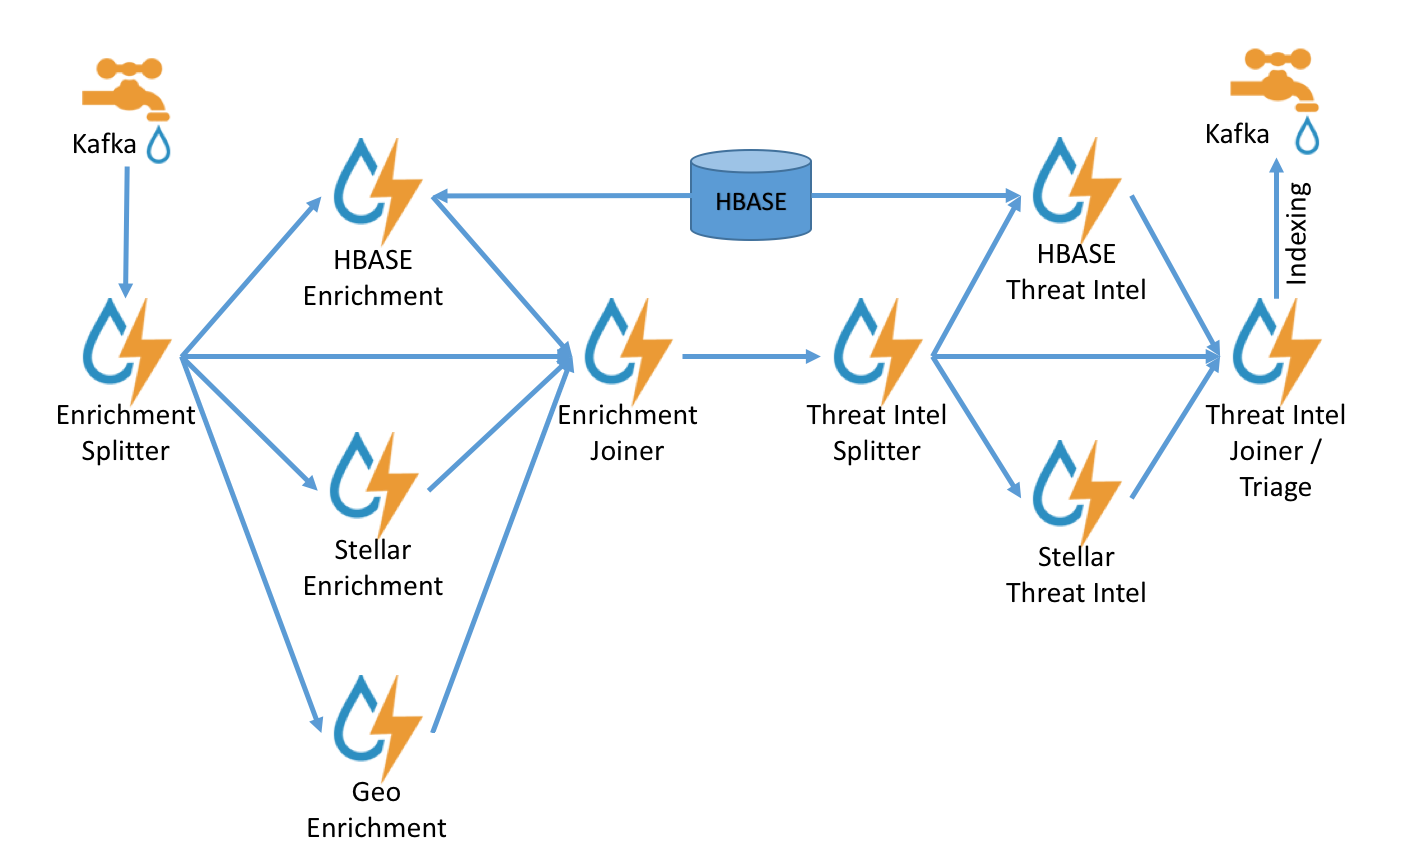
\includegraphics[scale=0.35]{images/enrichment_arch.png}}
\end{center}
}

\frame{\frametitle{Enrichment: New Hotness}
\begin{center}
  \makebox[\textwidth]{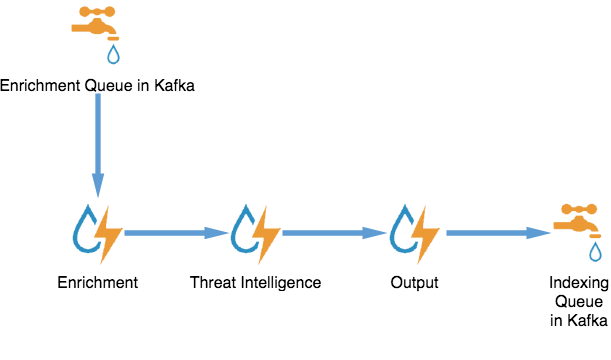
\includegraphics[scale=0.35]{images/enrichment_arch_new.png}}
\end{center}
}

\frame{\frametitle{Kappa Is a Great Tool But a Poor Master}
  \begin{itemize}
    \item We started with a Kappa architecture\pause
    \item Pretty much immediately we were asked to rerun data in batch
  \end{itemize}
}

\frame{\frametitle{If you take away three things from this talk...}
  \begin{itemize}
    \item Monitor, monitor, monitor\pause
    \item Streaming analytics, marriage and diplomacy are exercises in compromise.\pause
    \item Effective streaming analytics is about bringing to bear as much context into the data streaming by as you possibly can computationally.  Find compromises accordingly.\pause
  \end{itemize}
}
\frame{\frametitle{Questions}
Thanks for your attention!  Don't forget to come to the cybersecurity Bird of a Feather session Thursday.
\begin{itemize}
\item Find me at http://caseystella.com 
\item Twitter handle: @casey\_stella 
\item Email address: cstella@hortonworks.com
\end{itemize}
}

\end{document}
